\chapter{Development of Metagenomic Sequencing Workflow}
\label{ch:Results1}
\textit{This chapter describes the development of an enrichment-based metagenomic sequencing workflow for application to plasma samples from individuals with sepsis due to community acquired pneumonia.}

\startcontents[chapters]{\vspace{-1.4cm}}
\singlespacing
\printcontents[chapters]{}{1}{\section*{ }\setcounter{tocdepth}{1}}
\doublespacing

\section{Introduction}
We anticipated two main challenges associated with metagenomic sequencing from sepsis plasma samples. Firstly, sensitivity for detecting microbial nucleic acids would be low since human nucleic acids would be present in greater excess, especially with antimicrobial use prior to sample collection. Secondly, the design of a single library preparation method suitable for sequencing both DNA and RNA when almost all examples of library preparation methods in the literature target only one type of nucleic acid. These challenges were addressed through the application of probe-based enrichment and a combined DNA and RNA library preparation workflow, respectively and we termed this probe-based targeted enrichment method \textit{Castanet}.

\subsection{Probe-based enrichment} 
Our starting point for targeted metagenomics using oligonucleotide enrichment probes was work done \parencite{Bonsall2015} by the Stratified Medicine to Optimise the Treatment of Patients with Hepatitis C Virus Infection (STOP-HCV) consortium (led by Professor Ellie Barnes, University of Oxford). The genome of Hepatitis C virus (HCV) is highly diverse with strains subdivided into seven genotypes which differ at approximately 30-35\% positions across the ~9650 nt genome. This makes work on HCV highly applicable its genomic diversity is analogous to the range of diverse bacteria and viruses we would need to target in CAP.

Bonsall and colleagues observed greater than 10$^{3}$ fold enrichment in mid-range viral load samples (10$^{4}$-10$^{5}$ IU/ml). This degree of enrichment enabled an increased depth of sequencing to be achieved, enabling more affordable sequencing through multiplexing of larger numbers of samples for the same amount of sequencing capacity.

In addition, the STOP-HCV group were able to exploit a phenomenon they observed, namely that a 20\% divergence between probe and target was tolerated with minimal reduction in enrichment efficiency. They started with a probe panel covering 4 genotypes and augmented it to improve coverage for the four already-included subtypes and six additional subtypes. To do this, a consensus sequence for each HCV subtype was generated. Then, for each whole genome sequence in a reference set, genomic regions with less than 80\% identity to a starting panel of probes were identified. For each of these regions, the subtype consensus sequence was considered as a reference if there was $\geq$ 80\% similarity. If not, a probe was added to cover that genomic region. In this way, a cost-effective, non-redundant set of probes was generated.

\subsection{Ribosomal multilocus sequence typing}
The ribosomal multilocus sequence typing (rMLST) scheme \parencite{Jolley2012} for combined taxonomy and typing in bacteria is a development from 16S rRNA gene approaches \parencite{Woese1987}. This approach indexes variation of the 53 bacterial ribosome protein subunit (\textit{rps}) genes to enable resolution into groups at all taxonomic and most typing levels. This is possible as the \textit{rps} genes are conserved enough to enable taxonomic organisation and yet sufficiently diverse to enable species and type characterisation. As of 23 July 2019, the rMLST database (http://pubmlst.org/rmlst) contained 304,876 genomes and 1,861,484 alleles. 

The rMLST scheme can be applied to the generation of an efficient panel of probes which enable species/type characterisation without coverage of the whole bacterial genome. In addition, the targeting of conserved regions means that probes are able to capture bacterial organisms despite intra-species genomic variation.

\subsection{Library preparation methods for metagenomics}
There are few examples in the literature of a single combined library preparation workflow suitable for the metagenomic sequencing of both DNA and RNA. A 2018 review \parencite{Forbes2018} details 65 peer-reviewed studies of diagnostic clinical metagenomics. The majority of studies describe sequencing-based techniques applied only to DNA-based or RNA-based genomes with a few examples describing parallel RNA and DNA workflows \parencite{Langelier2018}, \parencite{Salzberg2016}. Only one small study (n=6) \parencite{Doan2016} successfully sequenced reads from DNA and RNA viruses (as well as fungi and parasites) from ocular fluid using a single protocol. This involved nucleic acid extraction, cDNA synthesis, and subsequent processing using the Illumina Nextera DNA Library Prep kit.

Other examples of combined library preparation methods include that described in the VirCapSeq-VERT method \parencite{Briese2015} which involved nucleic acid extraction, cDNA synthesis, fragmentation using ultrasonication, and subsequent processing using the KAPA library prepration kit. However, the authors did not trial this method on actual clinical specimens. 

\subsection{Viral multiplex reference}
We evaluated our workflow using a Viral Multiplex Reference (VMR) control (11/242) available through the UK National Institute for Biological Standards and Control (NIBSC). The reagent contains 25 viruses covering a range of genome types (dsDNA, dsRNA, ssRNA+, ssRNA-), sizes (6.8-233.7 kb), envelope types and pre-assayed concentrations (Table ~\ref{tab:VMR}). The viruses represent a range of common hazard group 2 human viruses (UK Advisory Committee on Dangerous Pathogens classification) and were propagated in cell culture or by egg passage, or isolated from clinical specimens.

Mee and colleagues \parencite{Mee2016} document a study involving 15 laboratories who were invited to process the VMR control using their own wet-lab and informatics methods. In this study, 6/25 target viruses were detected by all laboratories and two laboratories detected all 25 viruses. We will compare the performance of \textit{Castanet} against these 15 laboratories.

\subsection{Aims}

\begin{enumerate}
	\item To use probe-based enrichment to increase sensitivity for sequencing organisms relevant to sepsis from CAP
	\item To optimise a library preparation method suitable for sequencing both DNA and RNA-based organisms from plasma
	\item To evaluate performance of the library preparation with enrichment against a known positive control reference set
\end{enumerate}

\section{Results}

\subsection{Probe panel development}
Development of the probe panel was performed in collaboration with the Childhood Meningitis and Encephalitis Study (ChiMES) group. We compiled a list of viral and bacterial pathogens relevant to paediatric meningitis and adult sepsis from CAP in the UK (Table ~\ref{tab:ProbeSetViruses}; Table ~\ref{tab:ProbeSetBacteria}). We also included several pathogens of current interest during the time of probe set development (Zika virus, Chikungunya virus). Considering the number of distinct entries on our list (116, from 17 virus families and 35 bacterial species) and the criteria for inclusion, we inferred that any omissions of a priori less likely organisms, including relevant fungal or parasite pathogens, would comprise rare ($<$1\% frequency) or novel and therefore unsuspected causes of meningitis or pneumonia and sepsis. We also included probes to 4 spike-in control sequences for methodological evaluation of \textit{Castanet}.

We targeted similar lengths of genomic sequence for each pathogen to achieve a comparable assay sensitivity, optimising the breadth of pathogens we could target and avoiding bias in favour of larger genomes. For each of the viruses, we downloaded from NCBI RefSeq the full set of complete genomes available at 1st August 2015. We constructed genome alignments using MAFFT from which to design the probes. For each of the included herpesviruses, whose genomes exceed 100 kbp, this involved a low-diversity region of ~20kb whilst for all other viruses we used the whole genome.  For bacterial species, we took advantage of the ribosomal multilocus sequence typing (rMLST) scheme, which targets 53 genes encoding ribosomal proteins present in all bacteria and resolves bacteria to a sub-species level, extracting relevant sequences from the rMLST database on 11 December 2015. 

Probe design was carried out by Dr Azim Ansari. In previous work with HCV, it had been observed that sequence capture efficiency is preserved when probe and target sequences differ at up to 20\% of positions, and that exploiting sequence similarity to avoid redundancy can make probe design substantially more efficient without sacrificing performance. Accordingly, for each sequence alignment we constructed a tree using pairwise distances, within which we identified clusters such that all sequences were less than 5\% divergent from one another. The 5.86 x 10$^6$ bases of cluster consensus sequences were used to design a panel of 52,101 Agilent SureSelect, 120 nucleotide RNA probes on the complementary strand.


\subsection{Evaluation of four library prepration methods} \label{ssec:lib_preps}
We chose to perform this initial library preparation (library prep) development on plasma from patients infected with Hepatitis C Virus due to a previously established workflow with this sample type within the STOP-HCV consortium.

Four different library prep methods were compared in five HCV samples: (i) RNA; (ii) DNA; (iii) Combined with Fragmentation (CF. RNA method followed by DNA method); and (iv) Combined with no Fragmentation (CnoF; DNA method preceded by reverse transcription with random primers). To assess the suitability of each method for DNA and RNA-based pathogens, samples were spiked with an RNA (External RNA Controls Consortium Spike-In Mix, ERCC) and DNA positive control (dsDNA plasmid fragments). Following total nucleic acid extraction, the DNA and RNA content of each sample was assayed (Agilent 2100 Bioanalyser platform). This enabled us to spike in the plasmid DNA and ERCC RNA and 3\% and 1\% concentration by mass respectively. There was no enrichment stage in these experiments.

Sequencing yielded a mean total read count of 1.5x$10^6$ (range 0.9-2.6x$10^6$) across the five HCV samples and four library preps with the majority of sequences aligning to the human reference genome (mean 95.6\%; range 91.5-99.1\%). Libraries following RNA prep were significantly lower in cDNA concentration, requiring volumes for equimolar pooling in excess of the other three methods by an average of 16-fold. Unsurprisingly, following the DNA prep method, no reads aligning to RNA sequences (HCV or ERCC) were identified in any sample (Figure ~\ref{fig:Fig4libprep}). These observations indicate that neither the RNA nor DNA prep in isolation would be suitable for the sequencing of sepsis samples. Thus, the remainder of this chapter concentrates on comparing the two combined library preps.

HCV yield was highest in the CnoF prep, superior even to the standard RNA library prep method used by the STOP-HCV group (Figure ~\ref{fig:Fig4libprep}c and d). The CnoF prep also yielded a higher percentage of reads mapping to ERCC than the other three methods (Figure ~\ref{fig:Fig4libprep}a). However, the CF prep was superior to the CnoF prep in yield of DNA plasmid reads (Figure ~\ref{fig:Fig4libprep}b).

\FloatBarrier
\newpage
\begin{sidewaysfigure}[htbp]
\centering
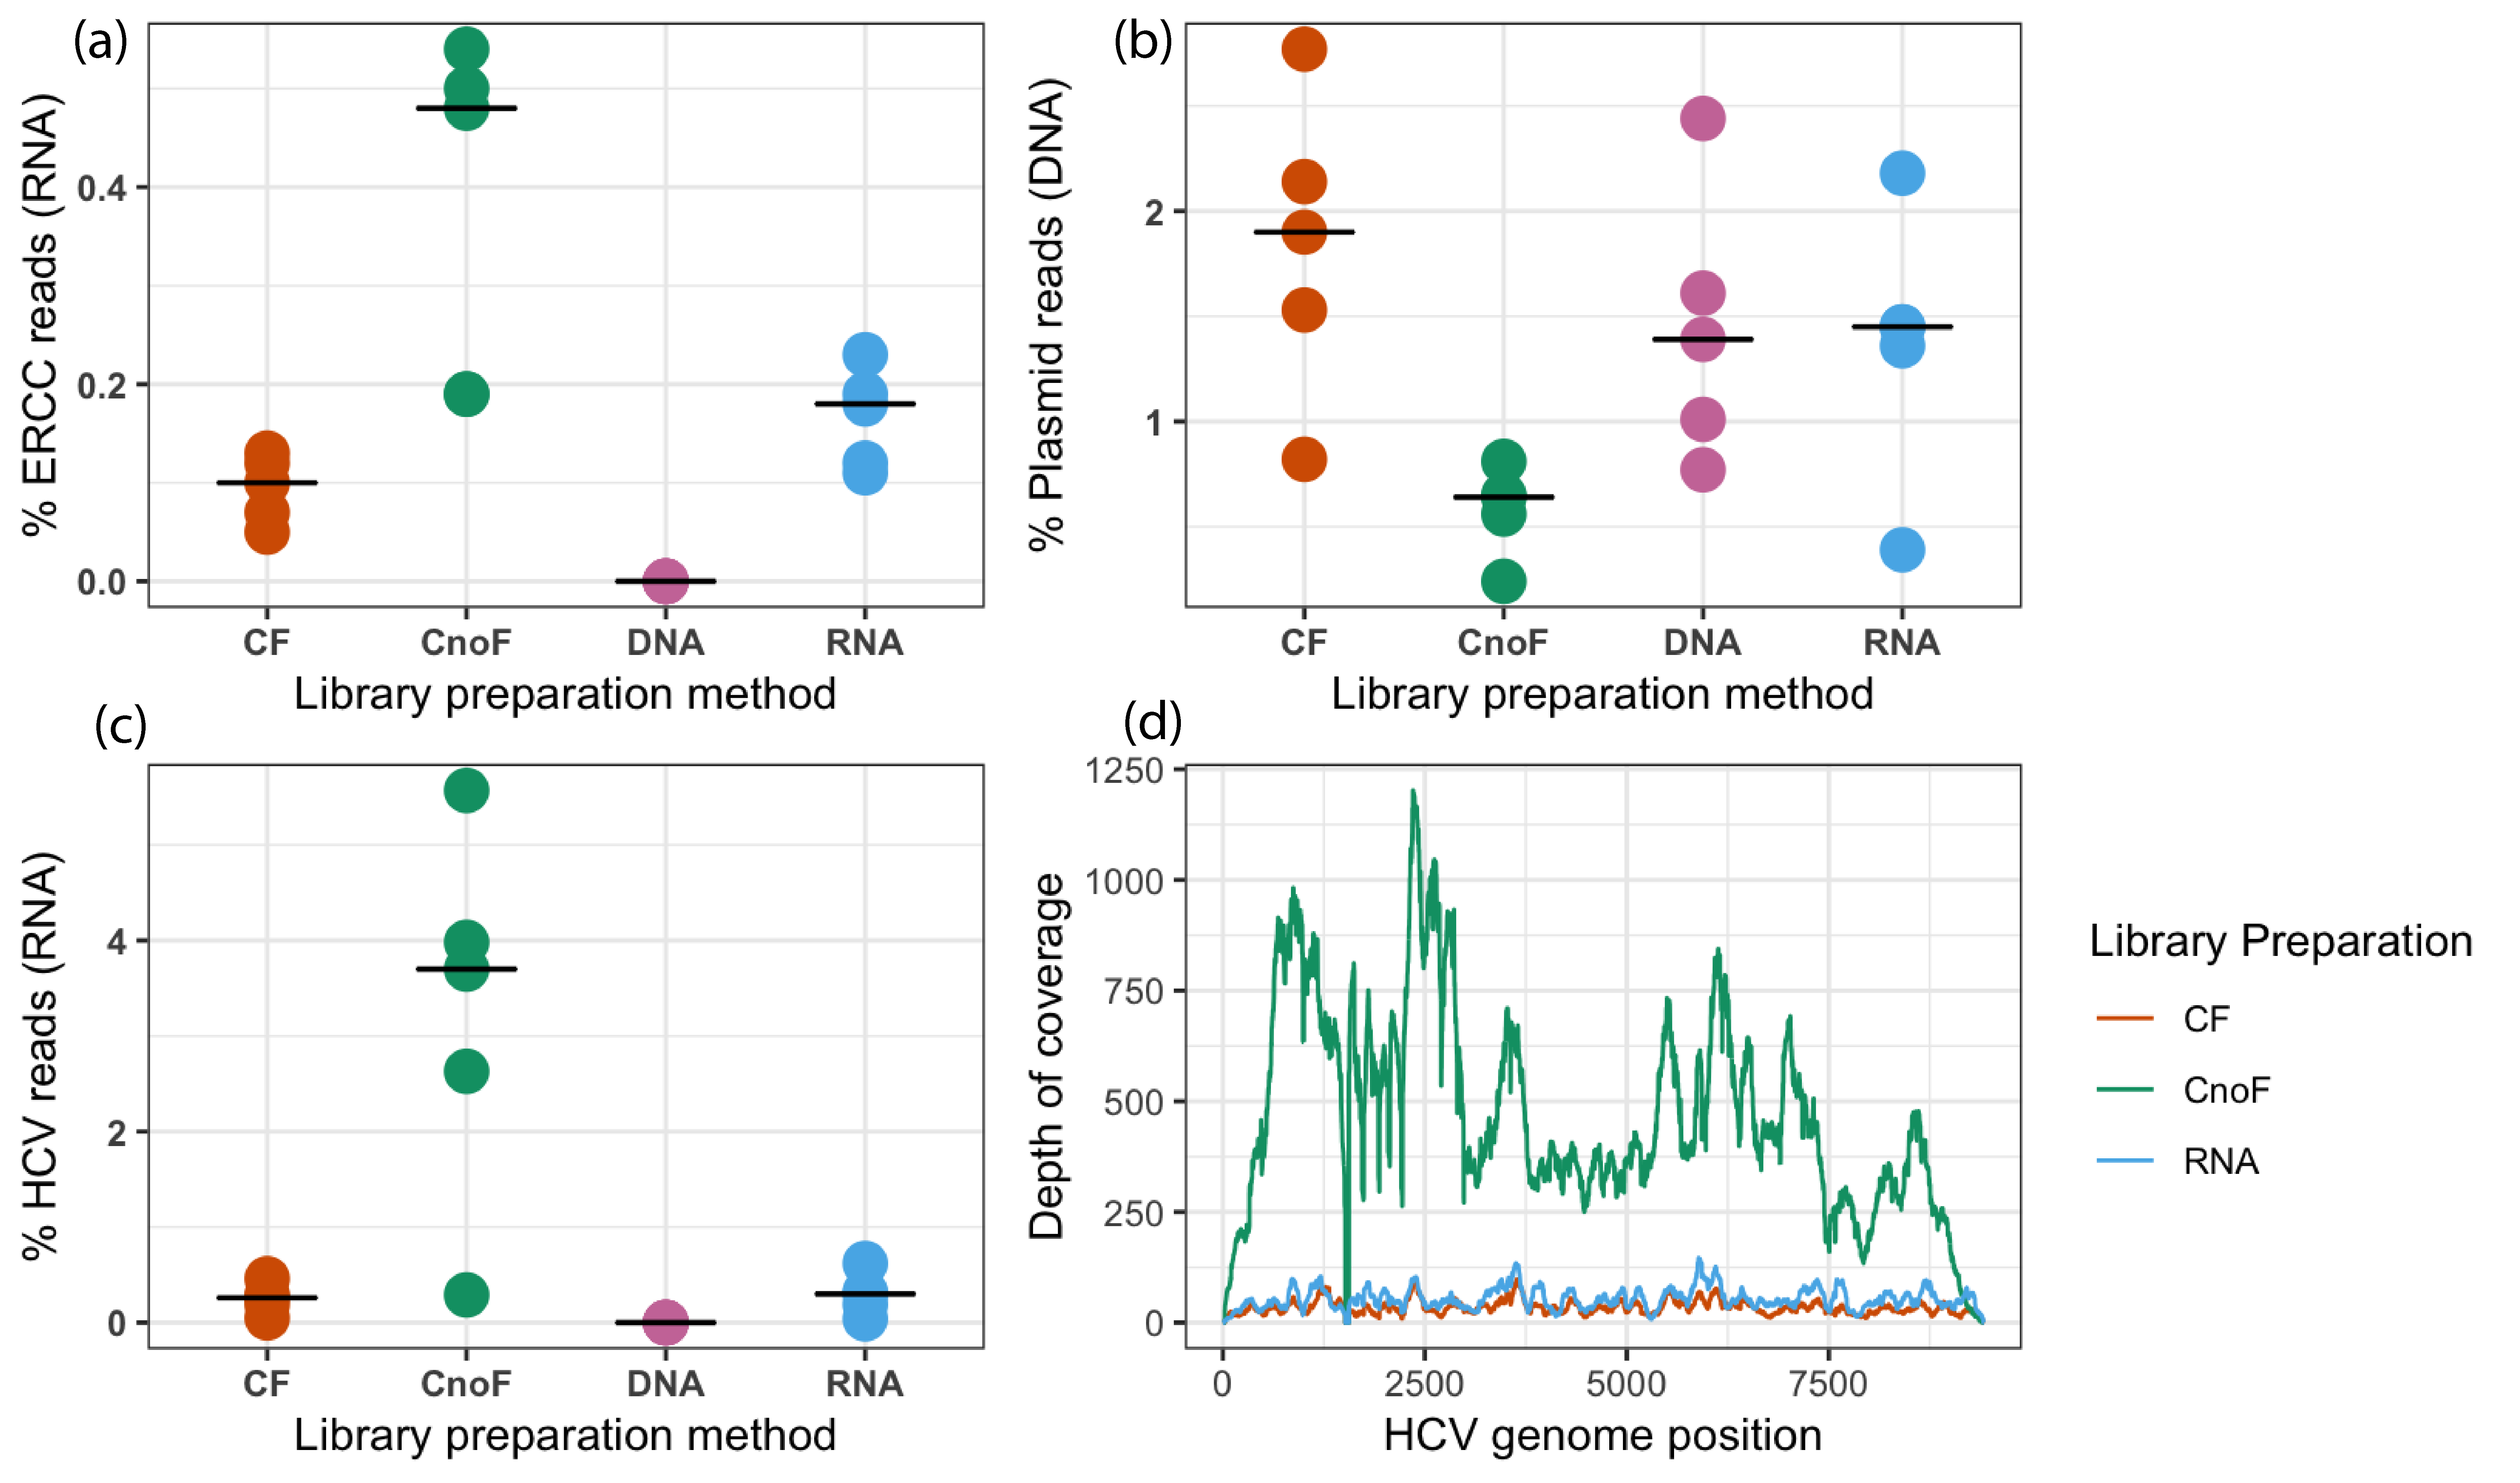
\includegraphics[width=\textwidth, scale=0.9]{./Results1/Images/libprep.png}
\caption[Comparison of four library preparation methods]{\textbf{Comparison of four library preparation methods} Plasma samples from five patients with HCV infection were processed by four library preparation methods in parallel. Performance of the different library preparation methods was evaluated with regards to: (a) ERCC RNA yield; (b) Plasmid DNA yield; (c) HCV RNA yield; (d) HCV genome coverage. (ERCC=External RNA Controls Consortium Spike-in Mix; CF=Combined with Fragmentation; CnoF=Combined with no Fragmentation; HCV=Hepatitis C Virus}
\label{fig:Fig4libprep}


\end{sidewaysfigure}
\FloatBarrier



For each sample, we calculated the input DNA:RNA spike-in ratio and compared this against the ratio of DNA:RNA (plasmid:ERCC) reads recovered (Table ~\ref{tab:plasmidERCC}). We observed that the yield of DNA:RNA reads closely matched the input spike-in concentrations of DNA:RNA with the CnoF prep, indicating that this method was similarly efficient for recovery of both DNA and RNA when compared to the CF prep.

\begin{table}[htbp]
\begin{center}
\begin{tabular}{|c|c|c|c|c|c|c|}
\hline
&& HCV1 & HCV2 & HCV3 & HCV4 & HCV5\\
\hline
Input & Both & 1.5 & 5.9 & 1.4 & 1.8 & 1.8\\
(Plasmid:ERCC mass) &&&&&&\\
\hline
Output & CF & 12.0 & 53.6 & 11.0 & 21.3 & 16.4\\
(Plasmid:ERCC reads)& CnoF & 1.1 & 4.2 & 1.3 & 1.3 & 1.2\\
\hline
\end{tabular}
\end{center}
\smallskip
\caption[Combined library preparations: plasmid to ERCC ratios]{\textbf{Sequencing yield of plasmid:ERCC reads relative to plasmid:ERCC spike-in mass}. The combined with no fragmentation (CnoF) and combined with fragmentation (CF) library preps are compared in plasma samples from five patients with HCV infection (HCV1 to HCV5)}
\label{tab:plasmidERCC}
\end{table}
\smallskip


\subsection{Evaluation of the Combined no Fragmentation protocol} 
A subsequent experiment was performed to further evaluate the CnoF library prep protocol (Figure ~\ref{fig:Exp2}), with the following specific aims: (i) to compare relative yield of reads originating from RNA and DNA; (ii) to evaluate the relationship of sequencing yield with read length and concentration for RNA and DNA; and (iii) to trial the CnoF protocol in sepsis patients. The sepsis samples were obtained from GAinS patients with sepsis due to CAP.

\begin{figure}[htbp]
\centering
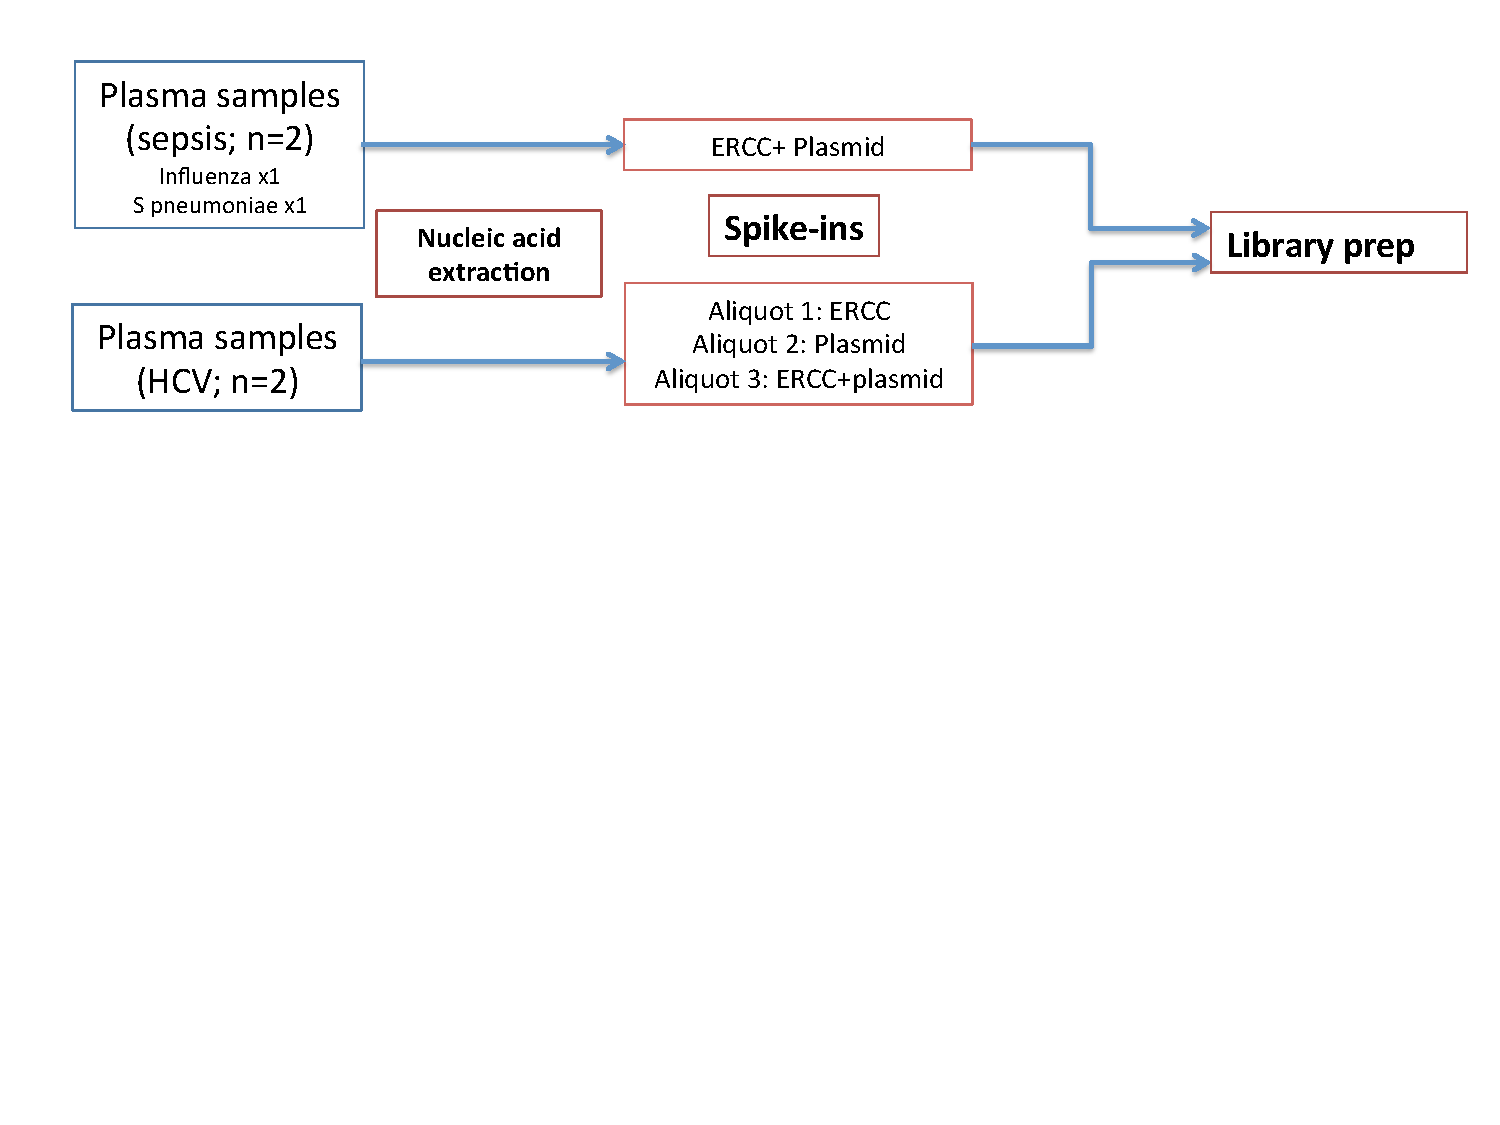
\includegraphics[width=150mm, trim={0 10cm 0 0},clip]{./Results1/Images/Exp2.pdf}
\caption[Combined no fragmentation library preparation evaluation]{\textbf{Workflow for CnoF Evaluation Experiment.} Each HCV sample was divided into three aliquots following nucleic acid extraction and spiked with (i) ERCC only, (ii) plasmid only, or (iii) both ERCC and plasmid. Each sepsis sample was spiked with both ERCC and plasmid.}
\label{fig:Exp2}
\end{figure}
\FloatBarrier

Sequencing yielded a mean total read count of 24.8x10$^6$ with minimal variation between HCV and sepsis samples (range 22.7-28.3x10$^6$) (Table ~\ref{tab:OptSummary}).

\begin{table}[]
\begin{tabular}{|c|c|c|c|c|}
\hline
                      & HCV2 & HCV4 & Sepsis1 & Sepsis2 \\ \hline
Total reads (x10$^6$) & 23.9   & 22.7   & 25.7    & 25.1    \\ \hline
\% Human              & 95.2   & 96.4   & 96.4    & 99.1    \\ \hline
\% HCV                & 1.98   & 0.44   & 0       & 0       \\ \hline
\% ERCC               & 0.23   & 0.27   & 0.20    & 0.18    \\ \hline
\% Plasmid            & 0.38   & 0.50   & 0.23    & 0.19    \\ \hline
\end{tabular}
\caption[Combined no fragmentation evaluation: summary]{\textbf{Percentage of reads aligning to each of the relevant reference genomes.} Results are for samples with dual ERCC and plasmid spike-ins. In this experiment, plasma samples from two patients with HCV infection (HCV2 and HCV4) and two patients with sepsis due to CAP (Sepsis1 and Sepsis2) was evaluated.}
\label{tab:OptSummary}
\end{table}

The proportion of reads mapping to the ERCC and plasmid references remained consistent whether the controls were spiked in individually or in combination, confirming that RNA was not impacting recovery of DNA or vice versa (Figure ~\ref{fig:spikein}). 

\begin{figure}[htbp]
\centering
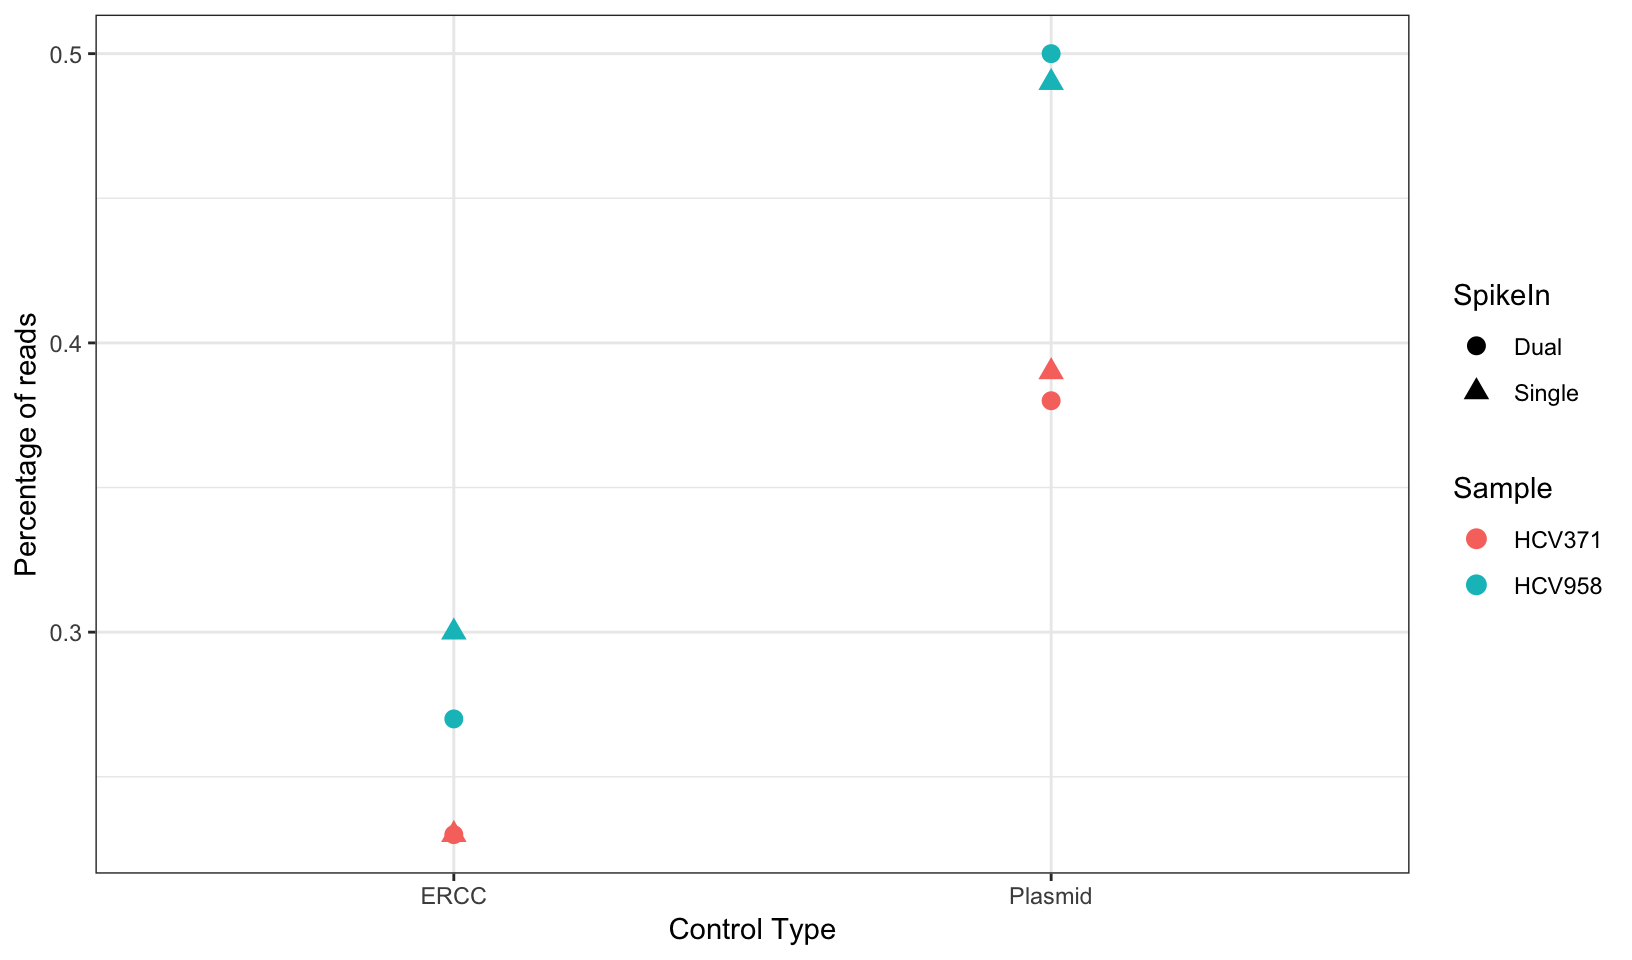
\includegraphics[width=12cm]{./Results1/Images/spike-ins-1.png}
\caption[Sequencing of spike-in controls]{\textbf{Sequencing yield of controls} Yield of ERCC and plasmid compared between aliquots receiving single and dual spike-ins}
\label{fig:spikein}
\end{figure}

The plasmid and ERCC controls were spiked-in at 1\% by mass of the initial sample DNA and RNA concentrations respectively. Thus, the relative mass ratio of plasmid to ERCC spike-ins varied between the samples. However, the ratio of plasmid to ERCC reads yielded reflected the input mass ratio fairly consistently between samples, indicating minimal bias towards RNA or DNA (Table ~\ref{tab:ratios}).

\begin{table}[]
\begin{tabular}{|c|c|c|}
\hline
Sample   & Input ratio (mass) & Output ratio (reads) \\ \hline
HCV2   & 1.94               & 1.65                 \\ \hline
HCV4   & 2.40               & 1.86                 \\ \hline
Sepsis1  & 1.12               & 1.15                 \\ \hline
Sepsis2 & 0.70               & 1.03                 \\ \hline
\end{tabular}
\caption[Combined no fragmentation evaluation: plasmid to ERCC ratios]{\textbf{Sequencing yield of plasmid:ERCC (reads) relative to spike-in input (mass).} The relative performance of the library preparation method for sequencing RNA and DNA was evaluated by comparing input to output ratios for plasmid:ERCC (DNA:RNA). Plasma samples from two patients with HCV infection (HCV2 and HCV4) and two patients with sepsis due to CAP (Sepsis1 and Sepsis2 was evaluated.}
\label{tab:ratios}
\end{table}


There was no association between sequencing yield and fragment size for either plasmid or ERCC (Figure ~\ref{fig:1bcontrollength}), indicating that the CnoF protocol performs consistently across the range of fragment sizes studied (plasmid 379-3190bp; ERCC 250-2000nt).

\begin{figure}[htbp]
\centering
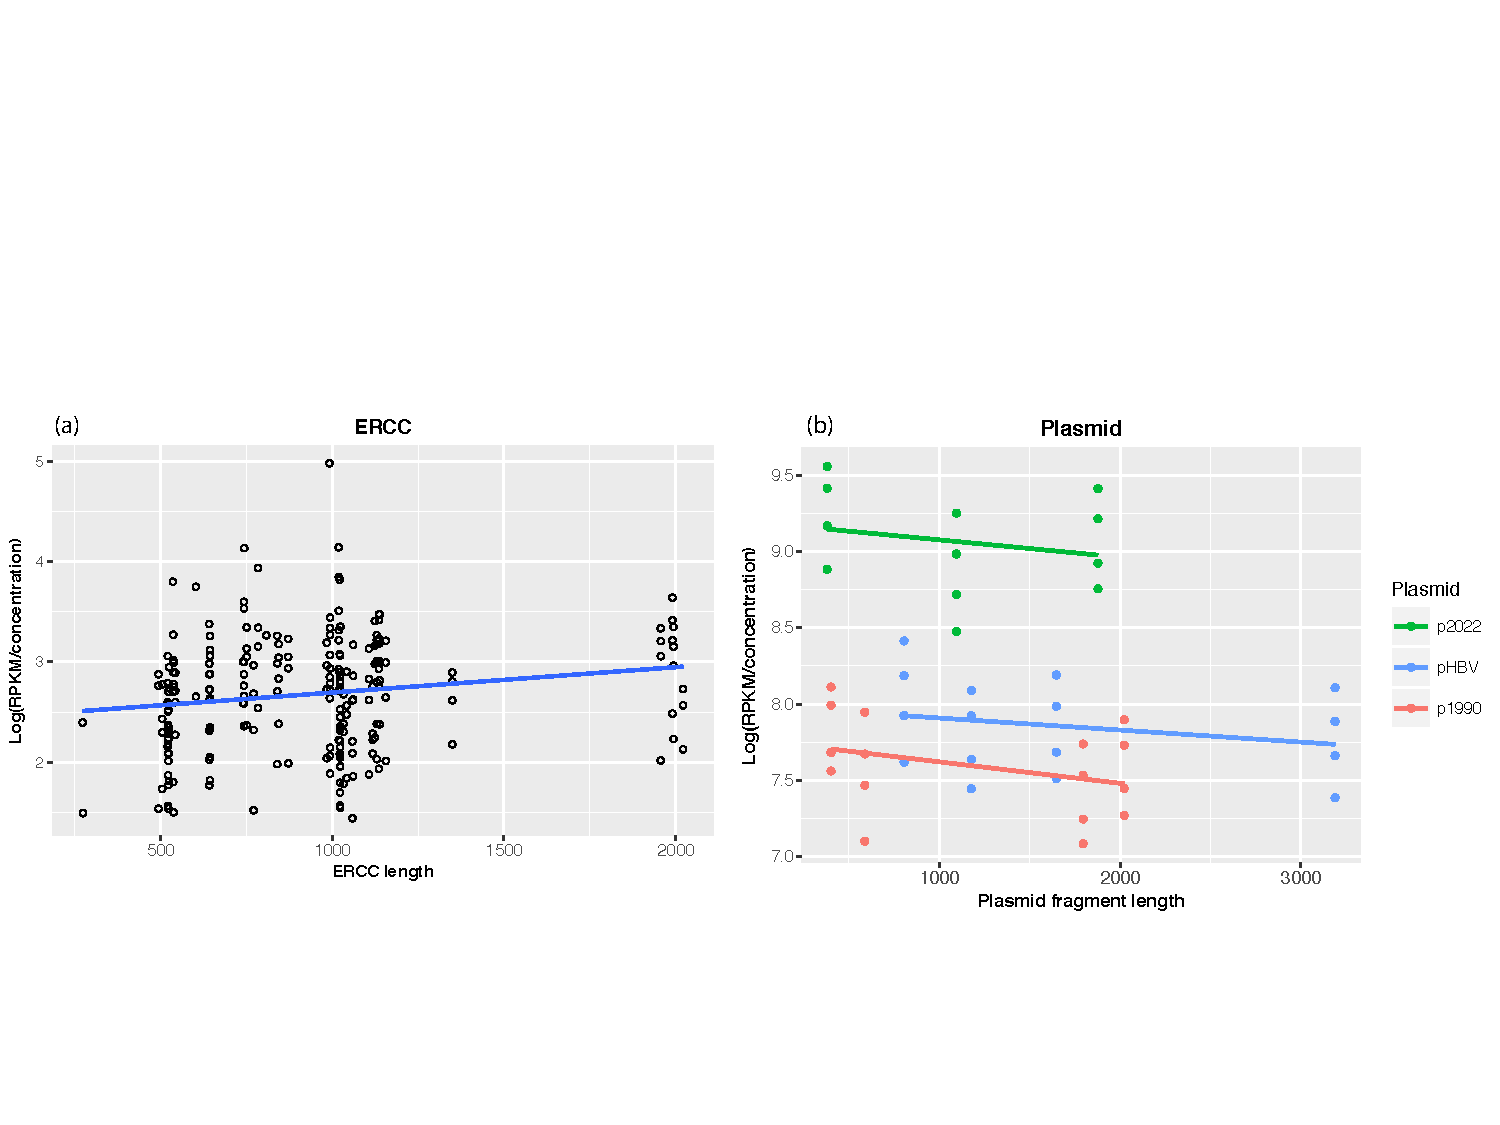
\includegraphics[width=\textwidth]{./Results1/Images/1b_control_length.pdf}
\caption[Relationship between read yield and fragment length]{\textbf{Relationship between read yield and fragment length.} (a) ERCC, (b) Plasmid. The y-axis displays read count normalised for fragment length, total read count per sample, and fragment concentration. RPKM = reads per kilobase of fragment per million reads.}
\label{fig:1bcontrollength}
\end{figure}



For the ERCCs, sequencing yield was proportional to input concentration (Figure ~\ref{fig:1bcontrolconc}). This association was less clear for the plasmid spike-ins. Although sequencing yield was highest for the p1990 plasmid (which was spiked-in at the highest concentration), the yield of p2022 was higher than that of pHBV despite a higher spike-in concentration of pHBV relative to p2022 (Figure ~\ref{fig:1bcontrolconc}). The differences observed between ERCC and plasmid probably reflect inaccuracies in plasmid nucleic acid quantification rather than differences between RNA and DNA processing in the library prep method. 



\begin{figure}[htbp]
\centering
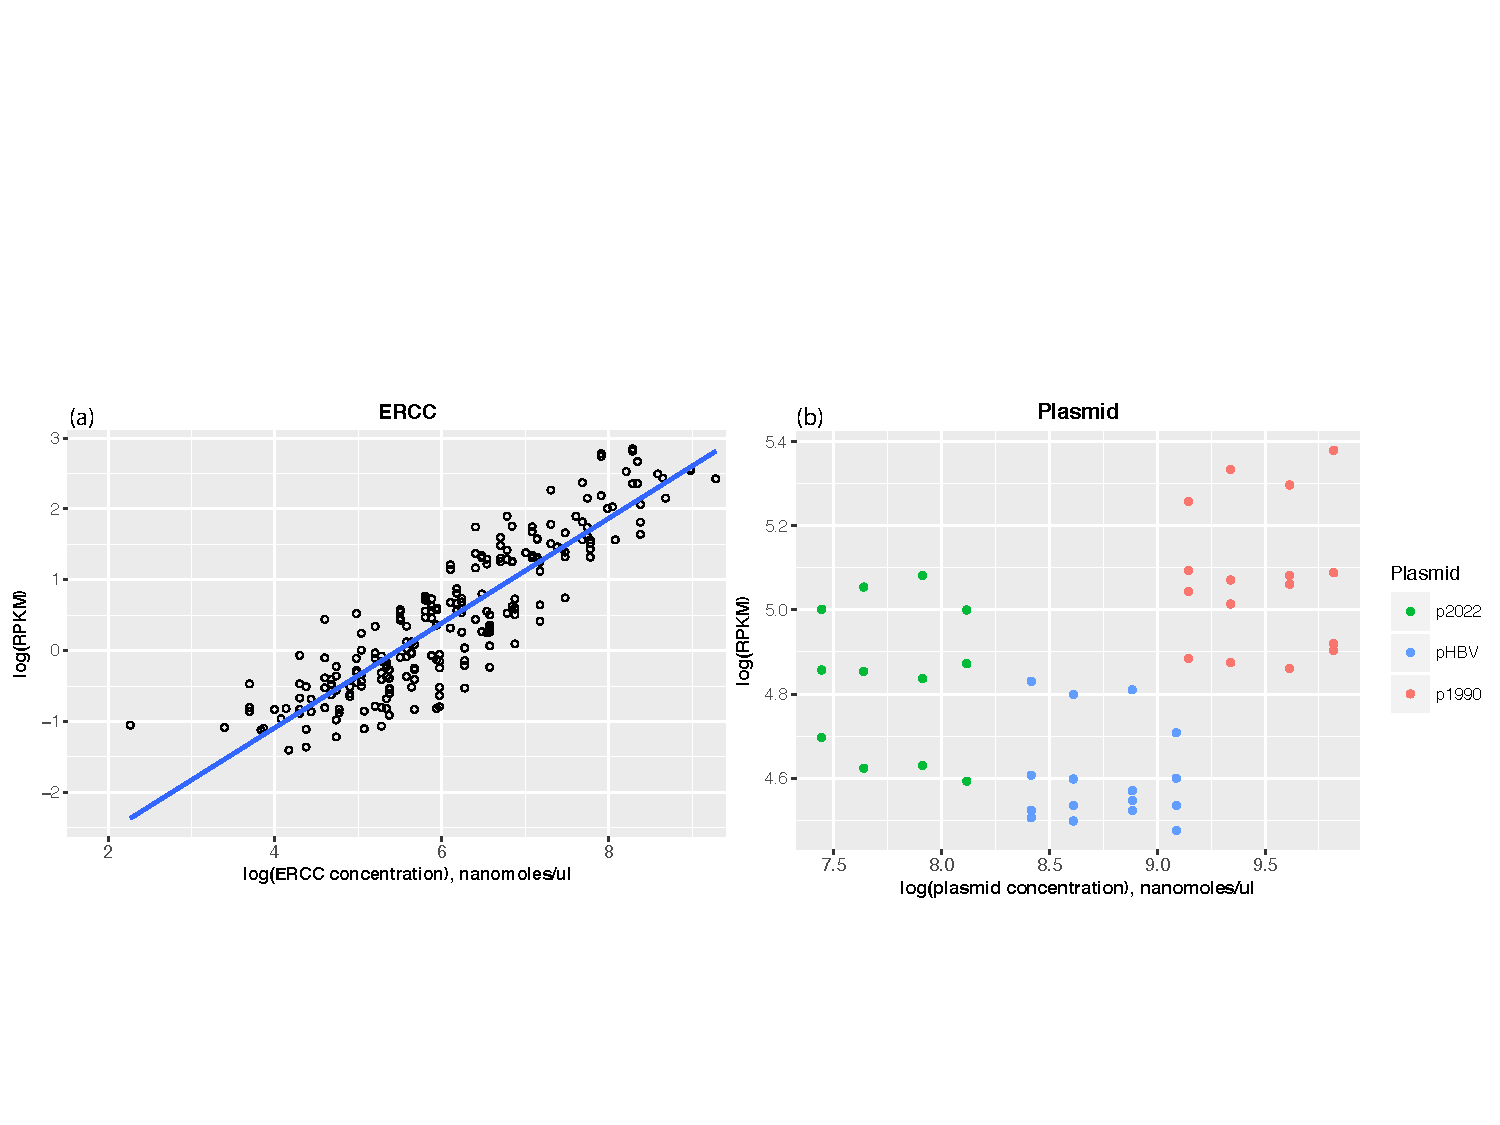
\includegraphics[width=\textwidth]{./Results1/Images/1b_control_conc.pdf}
\caption[Relationship between read yield and input concentration]{\textbf{Relationship between read yield and input concentration (molarity).} (a) ERCC, (b) Plasmid. RPKM = reads per kilobase of fragment per million reads.}
\label{fig:1bcontrolconc}
\end{figure}


Finally, we did not observe significant differences in total read count or recovery of spike-ins between plasma from sepsis patients compared to HCV patients.




\subsection{Evaluation of performance using a Viral Multiplex Reference control}
We combined four 1ml aliquots of reagent and made two replicates of a series of five dilutions (neat, 1:10, 1:100, 1:500, 1:1000) in phosphate-buffered saline solution, forming 500ul aliquots for extraction and library preparation. 

We used dilutions of a commercially available mixture of viruses (NIBSC Viral Multiplex Reference 11/242) to assess the quantitative range of detection of our method. For two undiluted VMR replicates, \textit{Castanet} sequencing yielded 9.1 and 10.9x10$^7$ reads. We detected all 21 viruses for which we had enrichment probes, with at least 8.65 reads per million in enriched samples, as well as two viruses not included (Sapovirus and Astrovirus; Figure ~\ref{fig:vmrheatmap}). Norovirus GI and GII were not detected; we did not have probes to capture this virus. A likely reason for this difference is that Sapovirus and Astrovirus were present in high enough concentrations to be sequenced without enrichment whilst Norovirus was present in lower concentrations. This is consistent with the 80\% failure rate in sequencing one or both Norovirus species in an evaluation of 15 laboratories with the same VMR control.

\begin{figure}[htbp]
\centering
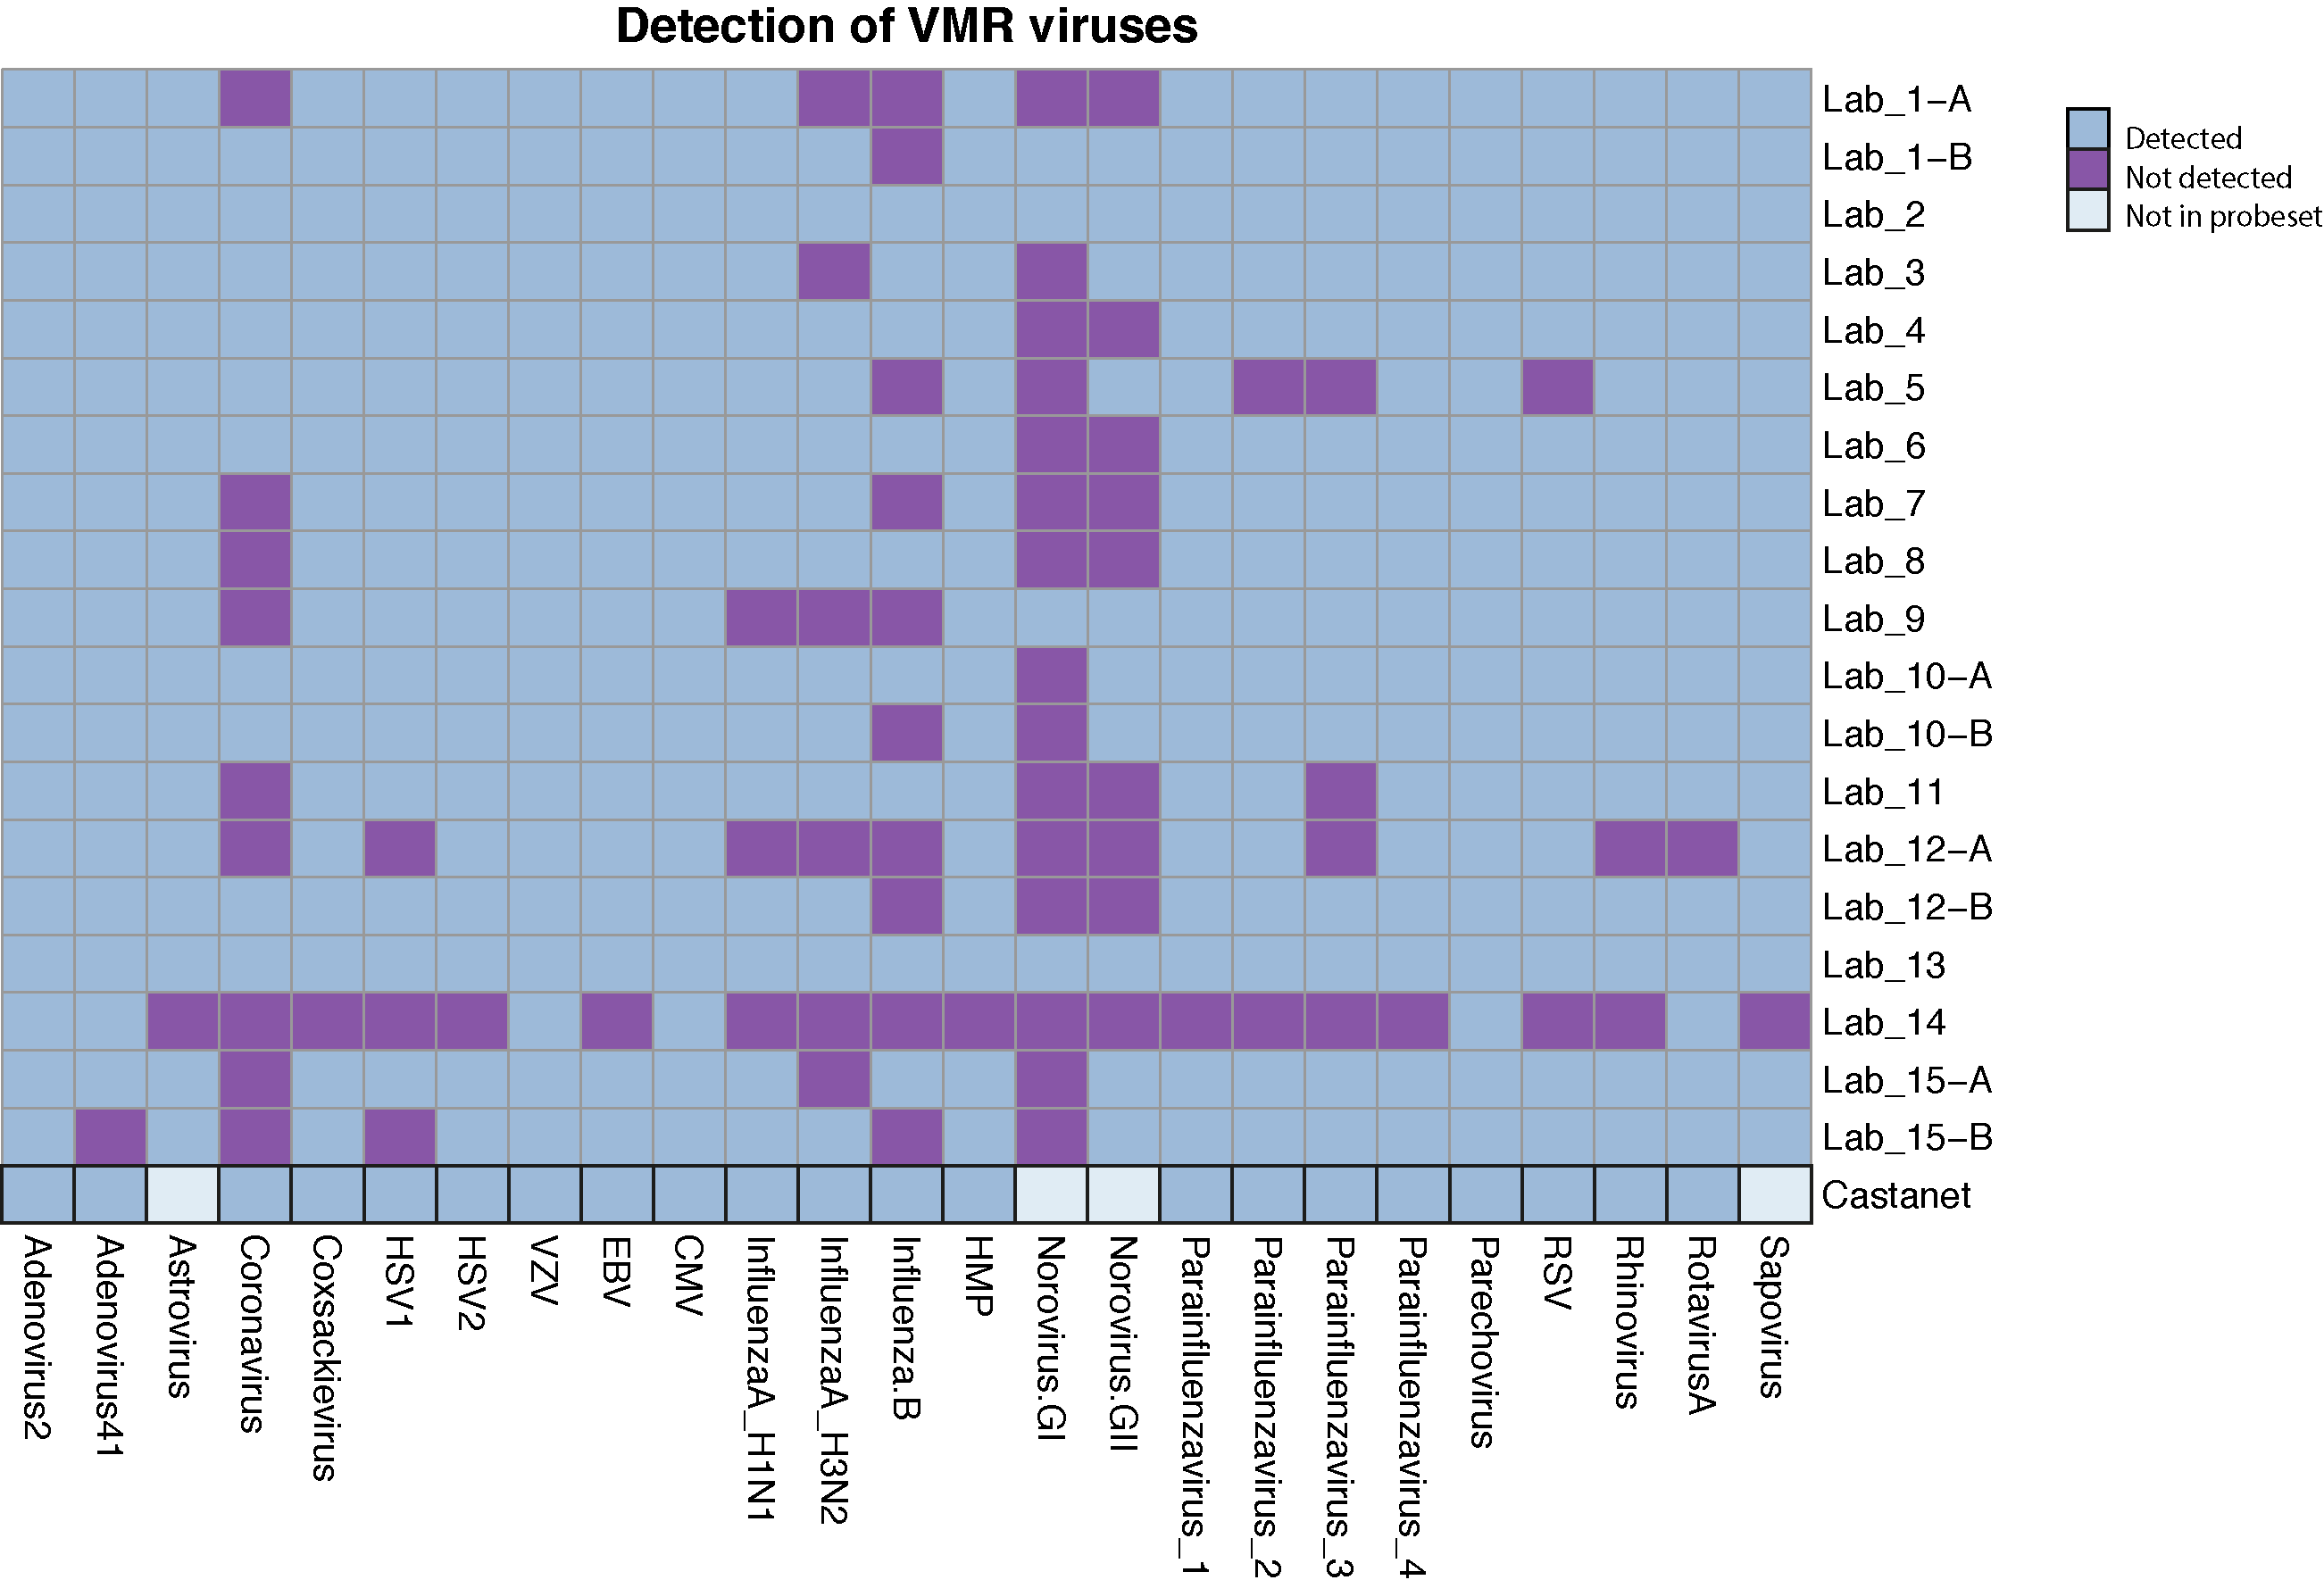
\includegraphics[width=\textwidth]{./Results1/Images/vmr-heatmap.png}
\caption[Viral Multiplex Reference Heatmap]{\textbf{Comparison of Castanet with 15 other laboratories for sequencing of viruses in the NIBSC Viral Multiplex Reference 11/242.} Mee and colleagues document the performance of 15 laboratories in sequencing the 25 viruses in the VMR. HSV=herpes simplex virus; VZV=varicella zoster virus; EBV=Epstein-Barr virus; CMV=cytomegalovirus; HMP=human metapneumovirus; RSV=respiratory syncytial virus}
\label{fig:vmrheatmap}
\end{figure}

For individual microorganisms, we observed a linear relationship between organism load and sequencing yield. The VMR included five viruses where viral load had been quantified by the NIBSC using qPCR. For each virus, the number of deduplicated reads was proportional to input concentration across the dilution series (neat, 1 in 10, 1 in 100, 1 in 500, 1 in 1000) (Figure \ref{fig:vmrconc}). However, the relationship between input viral load and yield of deduplicated reads differed between viruses. We observed a 10$^2$-10$^3$-fold enrichment for the five quantified viruses (Figure \ref{fig:vmrenrich}).

\FloatBarrier
\begin{figure}[htbp]
\centering
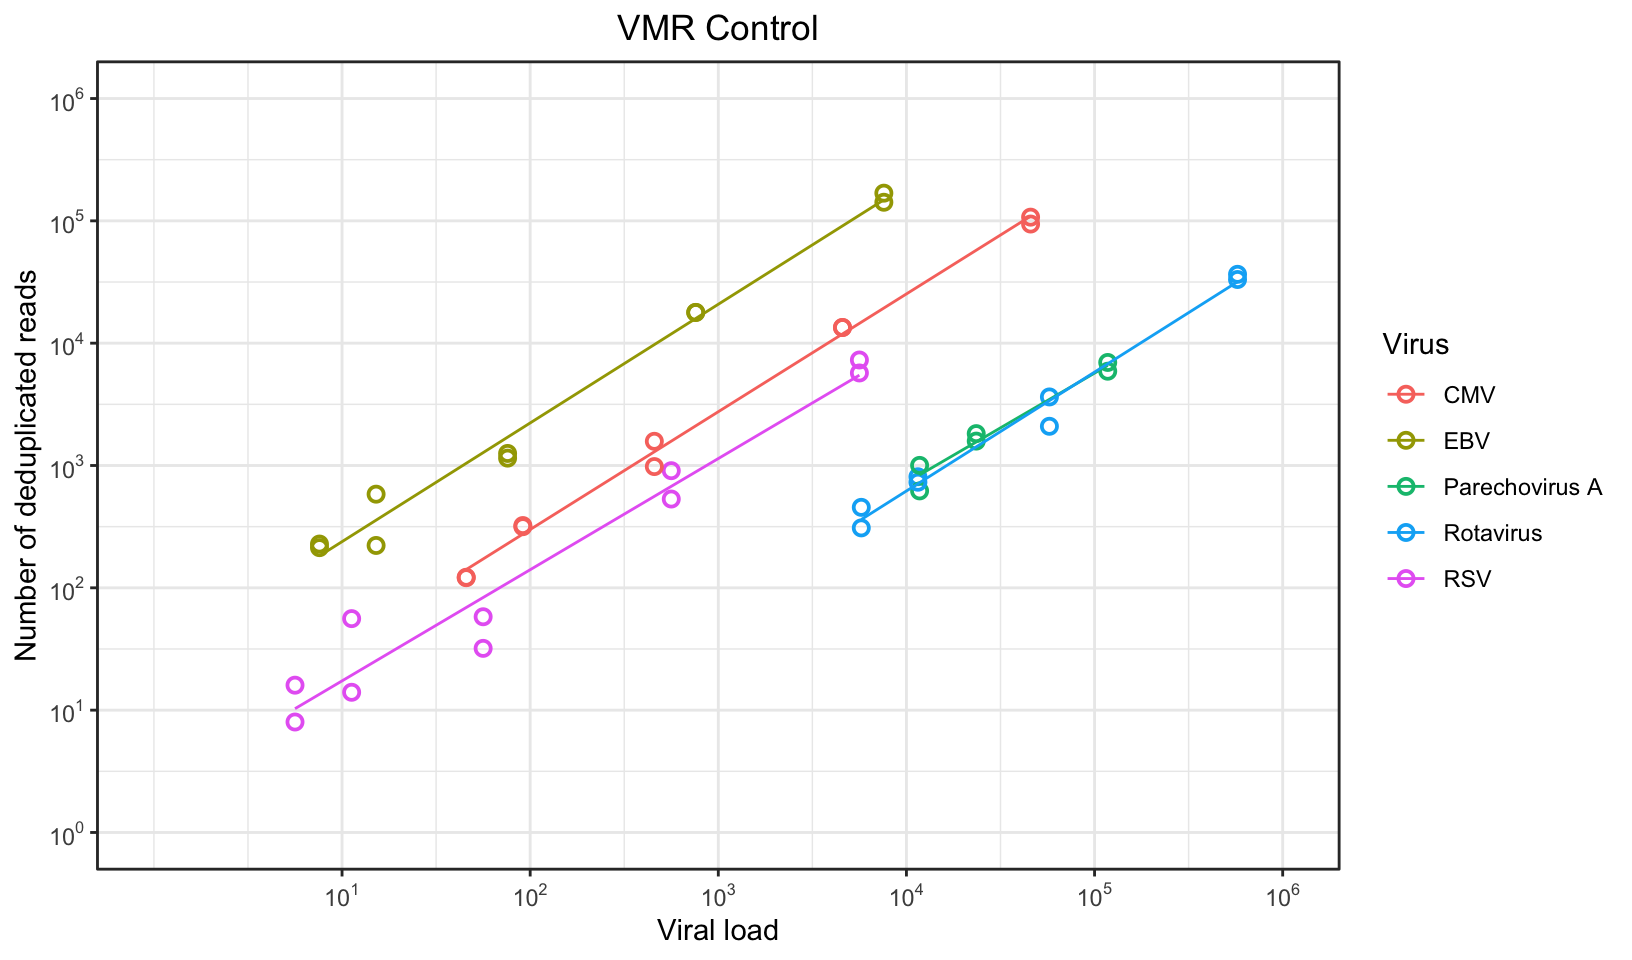
\includegraphics[width=\textwidth]{./Results1/Images/vmr-1.png}
\caption[Viral Multiplex Reference ]{\textbf{Relationship between viral load and sequencing yield in Viral Multiplex Reference (VMR) samples.} The VMR was sequenced at a range of dilutions in two replicates. For the five viruses in the VMR that had been quantified by the NIBSC using qPCR, the relationship between viral load and sequencing yield is plotted. (CMV=cytomegalovirus; EBV=Epstein-Barr Virus; RSV=Respiratory Syncytial Virus)}
\label{fig:vmrconc}
\end{figure}
\FloatBarrier

 

\FloatBarrier
\begin{figure}[htbp]
\centering
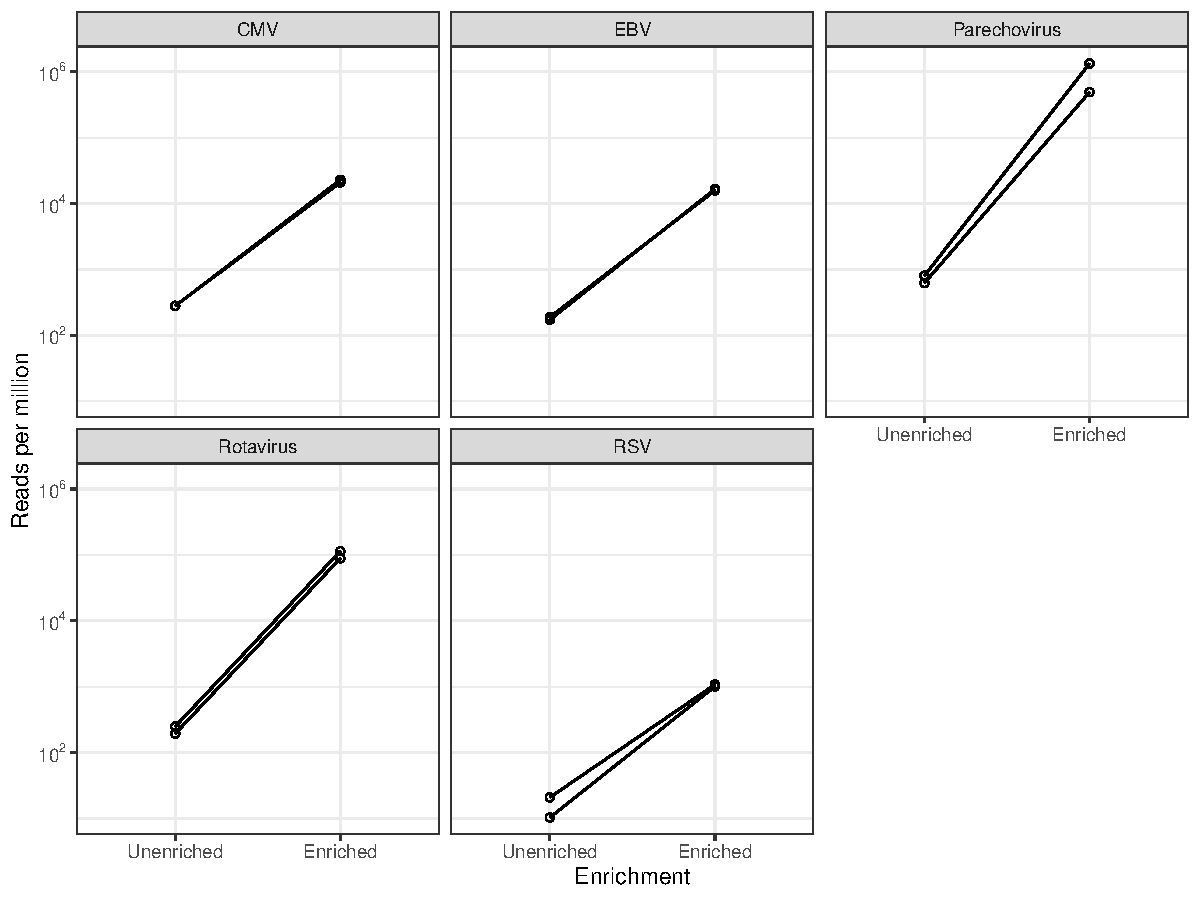
\includegraphics[width=\textwidth]{./Results1/Images/vmr-enrichment.pdf}
\caption[Viral Multiplex Reference Enrichment]{\textbf{Increase in sequencing yield with enrichment} The VMR was sequenced in two replicates at undiluted concentration. The sequencing yield (reads per million total reads) is plotted for each of the five viruses quantified by the NIBSC using qPCR. (CMV=cytomegalovirus; EBV=Epstein-Barr Virus; RSV=Respiratory Syncytial Virus)}
\label{fig:vmrenrich}
\end{figure}
\FloatBarrier

\subsection{Data processing}
A data processing pipeline (Figure \ref{fig:dataprocessing}) was developed in collaboration with Dr Tanya Golubchik from the ChiMES project. 

\FloatBarrier
\begin{figure}[htbp]
\centering
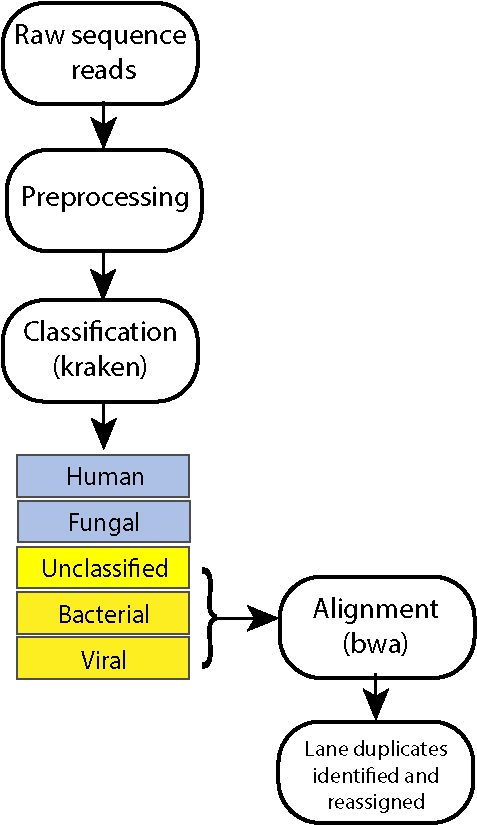
\includegraphics[width=0.5\textwidth]{./Results1/Images/data-processing.png}
\caption[Data Processing Pipeline]{\textbf{Data processing pipeline}}
\label{fig:dataprocessing}
\end{figure}
\FloatBarrier

De-multiplexed sequence read-pairs were trimmed of adapter sequences using Trimmomatic v0.36, with the ILLUMINACLIP options set to “2:10:7:1:true MINLEN:50”, using the set of Illumina adapters supplied with the software \parencite{Bolger2014}. The trimmed reads were then classified using Kraken v1 \parencite{Wood2014} using a custom database containing the human genome (GRCh38 build), all RefSeq bacterial and viral genomes, and a selection of fungal genomes that were most likely to be associated with cases of meningitis \parencite{Cuomo2017}. These were: \textit{Aspergillus fumigatus}, \textit{Candida} spp., \textit{Coccidioides} spp., \textit{Cryptococcus} spp., \textit{Histoplasma capsulatum}, \textit{Paracoccidioides brasiliensis}, and \textit{Pneumocystis} spp. This custom database including both human and microbial reads was created to optimise the accuracy of classification, minimising the likelihood of human reads being classified as microbial or vice versa.

Subsequently, reads identified by Kraken as bacterial or viral were aligned using BWA v0.7.1243 with default settings to a multi-fasta reference of consensus sequences corresponding to the enrichment probe targets, augmented with sequences of known or suspected contaminants. These included (i) reagent contaminants (\textit{Alteromonas} and \textit{Achromobacter} spp.), (ii) genomes of two viruses known to have been sequenced on the same flow cell: MVMPCG spike-in control and Echovirus 7; and (iii) the rMLST sequences of commensal Streptococcus species (\textit{S. mitis, S. oralis, S. pseudopneumoniae}) that were thought to be likely contaminants in clinical samples. This two step process of Kraken classification followed by BWA alignment has not previously been described; it was used in the \textit{Castanet} data processing pipeline as the initial Kraken step efficiently and accurately separates human/fungal from bacterial/viral reads, enabling the BWA mapping to occur in a computationally efficient manner, accurately aligning reads to the probe sequences. 

Following BWA alignment, we corrected our sequencing results for index misassignment (index hopping). This well-recognised phenomenon occurs when a small proportion of reads belonging to a sample gets misassigned to a different index in the multiplexed pool. For each sequencing pool, we identified duplicated reads and reassigned all reads in each duplicate cluster to the sample with the highest number of reads in that cluster. This data processing step is unique to \textit{Castanet} and decreases the number of false positives arising from index hopping.

After duplicate reassignment, we calculated a set of descriptive statistics for each sample and target organism. These included sequencing depth with and without deduplication, and coverage of target sequences at various depth thresholds. The collected statistics were combined with available laboratory data and ddPCR results where available and the resulting data frame used to train a random forest model (Section 4.2.1). 

\section{Discussion}
In this chapter, I have described \textit{Castanet}, a versatile probe-based enrichment sequencing method that combines the analysis of RNA and DNA from the same starting material in a single protocol and enriches for pathogens of interest using a modestly sized panel of probes.

\subsection{Combined library preparation method}
We developed a single library preparation workflow which combines separate RNA and DNA workflows in a single streamlined protocol, enabling the successful sequencing of both spike-in controls (ERCC and plasmid) as well as the VMR control. The experiments involving the spike-in controls were performed without enrichment whilst those involving the VMR control were performed with enrichment.

The CnoF protocol enabled sequencing of targets originating from RNA and DNA without bias, as evidenced by the yield of DNA:RNA closely matching input ratios of DNA:RNA for the plasmid (DNA) and ERCC (RNA) spike-in controls. This lack of bias is particularly important for detecting cases of co-infection in CAP, e.g. co-infection with DNA-based \textit{Streptococcus pneumoniae} and RNA-based influenza A virus. 

We also observed that there was no association between sequencing yield and fragment size for either plasmid or ERCC. This is important as it demonstrates a lack of bias towards particular fragment sizes, which could in theory preferentially favour the sequencing of one organism over another. However, the analysis is limited to the range of fragment sizes studied (plasmid 379-3190bp; ERCC 250-2000nt). 

For the five quantified viruses in the VMR, we observed a linear relationship between input concentration and sequencing yield. However, we noted that this relationship differed between viruses, presumably because of differences in the enriched (genomic) sequence length, the efficiency of sequencing library formation and capture and, perhaps the calibration of qPCR assays. Nevertheless, our results indicate that for a particular organism, deduplicated read counts can be compared between samples to provide information about relative organism loads. 

\subsection{Enrichment for targets of interest}
We developed a probe panel covering 116 organisms from 17 virus families and 35 bacterial species. Considering the extent of coverage, the size of the probe panel was modest at 5.86 x 10$^6$ bases, with minimal redundancy and associated cost savings. 

To my knowledge, this is the first published example of a probe panel that includes both bacteria and viruses as well as one targeting specific diseases. Other examples of probe panels include the separate bacterial BacCapSeq \parencite{Allicock2018} and viral VirCapSeq-Vert \parencite{Briese2015} panels which target all human pathogenic bacteria and vertebrate viruses respectively. 

As our probe panel was designed based on conserved \textit{rps} genes of the bacterial genome, there are several limitations. Firstly, we are unable to distinguish between different species of the Enterobacteriaceae family because of sequence homology within this region. Secondly, we did not enrich for regions encoding for virulence genes and antimicrobial resistance genes. Although we did not set out with the latter aim, future iterations of the probe panel would benefit from extending beyond the rMLST system.

We observed between a 10$^2$ to 10$^3$-fold enrichment for the five quantified VMR viruses. The two higher viral load viruses (Parechovirus, Rotavirus) showed higher fold-change enrichment (10$^3$-fold vs 10$^2$-fold) compared to the lower viral load viruses (CMV, EBV, RSV). This is in keeping with the observations of \parencite{Bonsall2015} who noted a 10$^3$ fold enrichment for mid-range viral load samples but lower fold-change enrichment for lower viral loads. 

\subsection{Data processing pipeline}
Our aim with the data processing was to implement a computationally efficient pipeline that would enable accurate alignment of microbial sequences. One challenge was the low signal to noise ratio, with the majority of samples containing $>$95\% human reads. We dealt with this by using kraken for classification prior to bwa alignment. By building a custom database with human and microbial reference sequences, we could identify the human sequences and discard them before BWA alignment, making the latter stage substantially faster.

Another challenge was contaminants, including those from kit reagents, patient skin/mucosa, and simultaneously sequenced samples. We dealt with this by adding these sequences to the multi-fasta file for alignment so that the contaminants would map to the correct references rather than mis-mapping to a closely related pathogenic organism. 

One area for future work is the diagnosis of fungal infections. Currently, we do not enrich for fungal reads and any sequences classified as fungal by kraken are discarded prior to BWA alignment. Fungal causes of CAP are currently underappreciated \parencite{Chen2001} and may represent a proportion of the cases which remain diagnosed after routine bacteriology/virology. 

\section{Conclusions}
In this chapter, I have described \textit{Castanet}, a targeted metagenomic approach using enrichment probes for the sequencing of DNA and RNA-based bacteria and viruses from patient samples. Here, I have evaluated \textit{Castanet} in terms of its performance for sequencing positive controls (plasmid and ERCC spike-ins; VMR control). In the next chapter, \textit{Castanet} is applied to a cohort of patient samples and further evaluated.

